\begin{picture}(0,0)%
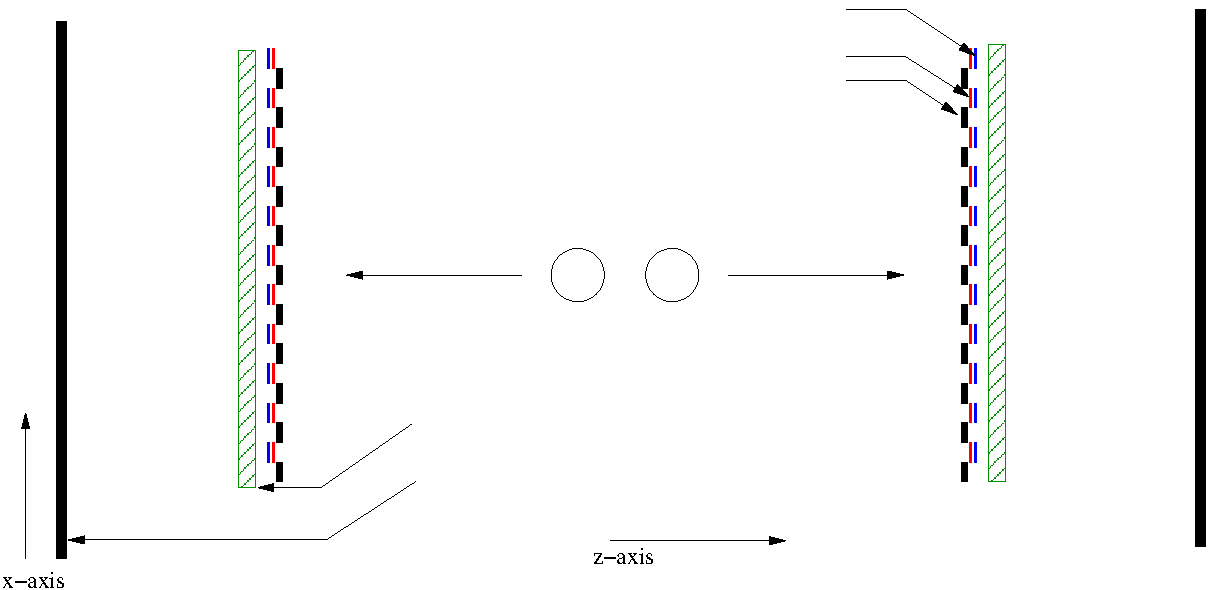
\includegraphics{/afs/tp.nt.uni-siegen.de/user/arora/Documents/projectSiegen/firstDraft/diagrams/scheme}%
\end{picture}%
\setlength{\unitlength}{4144sp}%
%
\begingroup\makeatletter\ifx\SetFigFont\undefined%
\gdef\SetFigFont#1#2#3#4#5{%
  \reset@font\fontsize{#1}{#2pt}%
  \fontfamily{#3}\fontseries{#4}\fontshape{#5}%
  \selectfont}%
\fi\endgroup%
\begin{picture}(9215,4490)(751,-4486)
\put(5431,-421){\makebox(0,0)[lb]{\smash{{\SetFigFont{12}{14.4}{\rmdefault}{\mddefault}{\updefault}{\color[rgb]{1,0,0}Birefringent Crystals}%
}}}}
\put(6121,-151){\makebox(0,0)[lb]{\smash{{\SetFigFont{12}{14.4}{\rmdefault}{\mddefault}{\updefault}{\color[rgb]{0,0,1}Glass slabs}%
}}}}
\put(6451,-691){\makebox(0,0)[lb]{\smash{{\SetFigFont{12}{14.4}{\rmdefault}{\mddefault}{\updefault}{\color[rgb]{0,0,0}Grating}%
}}}}
\put(4951,-1726){\makebox(0,0)[lb]{\smash{{\SetFigFont{12}{14.4}{\rmdefault}{\mddefault}{\updefault}{\color[rgb]{0,0,0}$\ket{\chi} = (\ket{HV} - \ket{VH})/\sqrt 2$}%
}}}}
\put(3916,-3616){\makebox(0,0)[lb]{\smash{{\SetFigFont{12}{14.4}{\rmdefault}{\mddefault}{\updefault}{\color[rgb]{0,0,0}Screen}%
}}}}
\put(3916,-3256){\makebox(0,0)[lb]{\smash{{\SetFigFont{12}{14.4}{\rmdefault}{\mddefault}{\updefault}{\color[rgb]{0,0,0}$45^o$ polarizer}%
}}}}
\end{picture}%
